\section{Introduction}

Since Sputnik was launched into space in 1957, humans have strived to be a spacefaring species. The international space race of the mid-20th century, particularly between the Unites States and the former Soviet Union saw quick succession of many space exploration milestones. Yuri Gagarin became the first man to reach outer space in 1961. In the same decade the Apollo 11 crew became the first men to walk on the Moon. Since then, space programs have sent countless science expirements, satellites, and probes across the Solar System. Largely due to tenuous funding and an uncertain purpose, space travel in the 21st century has been a quiet endeavor. The United States National Aeronautics and Space Administration (NASA) has largely been focused on robotic studies of other planets, developing advanced space technologies, and maintaining current infrastructure like the International Space Station (ISS) and the Hubble Space Telescope.

A once unachievable dream seems to be reigniting as scientists and the public discuss the potential for extraterrestrial deep space exploration, like that of Mars. As can be seen in Fig. \ref{fig:budget}, funding for space exploration research in Mars has stayed relatively constant while cumulative interest in deep space exploration has increased over the 21st century. Interest in space travel has recently been dominated by the desire to further scientific understanding of the universe and the commercial desire to extract extraterrestrial resources for use on Earth. Because of historical challenges in publicly funding space exploration, there has been an advent of private space companies funded by investors and enterprises like SpaceX, Virgin Galactic, and Blue Origin. The economic advantage of these companies is their ability to self-fund space technology and conduct contract work \cite{space-contract} with less reliance on public funding.

This renewed interest propelled by private companies is returning public interests to the focus of manned missions, moving beyond the currently common practice of using robots or satellite probes \cite{nasa-landers}. This effort seems most notable in SpaceX, who have very publicly expressed their interest in leading missions that culminate in permanent settlements on extraterrestrial bodies \cite{spacex-mars-press}. This unprecedented feat, if successful, would lead to a new era in human history that previously only lived in the realm of science fiction.

Even if public interest remains strong, this process will require significant strides ahead of current space technology. Manned missions require additional payloads for life-support that would normally not be required for deep space satellites. This extra payload means new rockets and propulsion systems are needed for sending astronauts on long journeys. NASA has detailed its expectations for novel and exotic space propulsion systems, including when they are expected to be viable \cite{nasa-propulsion}. Among the potential systems are spacecraft driven by nuclear reactors. If these advancements in technology occur on an expected timeline, they may coincide with intended roadmaps for deep space exploration projects. Regardless of what innovative technology ends up being used, any manned spacecraft will require shielding to protect humans from the biological effects of space travel, particularly harmful radiation. This paper presents a literature review on the existing research and requirements for designing spacecraft suitable for human deep space exploration. Reviews of the biological effects of space radiation and the existing shielding strategy for spaceship design are included. Finally, some technologies are highlighted for their novel potential for advanced spacecraft functionality.

\begin{figure}
\centering
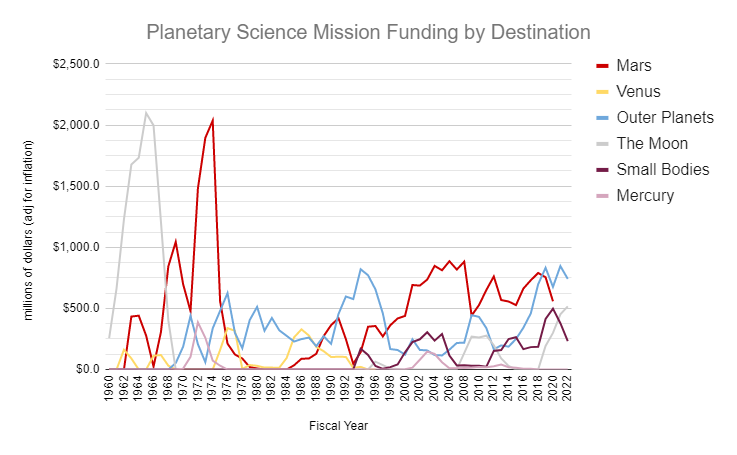
\includegraphics[width=\linewidth]{mars-budget.png}
\caption{Mission funding for planetary space exploration created by the Planetary Society \cite{planetary-society}. While planetary funding peaked during the space race of the 20th century, there has been a recent increase in cumulative planetary exploration funding. While Mars funding has stayed relatively constant in the past two decades, it has consistently been a planet of significant interest to public agencies.}
\label{fig:budget}
\end{figure}
